\chapter{Možnosti rozšírenia}
V tejto kapitole sa pozrieme na rôzne možnosti a smery, akými by sme mohli našu aplikáciu ďalej rozšíriť.
\section{Ukladanie výstupu do súboru}
Niektoré analyzátory ponúkajú ukladanie výpisu do rôznych súborov. V prípade ak by sme sa rozhodli našu aplikáciu rozšíriť o možnosť ukladania analýzy do súboru, museli by sme si rozmyslieť niekoľko nasledujúcich vecí:

\paragraph{Formát výpisu}
\hfill \break
Akým spôsobom bude vyzerať výstup analýzy. Na výber máme viacero možností od obyčajného textového výstupu až po obrázky alebo rôzne tabuľky. Na začiatok by nebolo príliš zložité zaintegrovať výpis analýzy v textovom formáte. Všetky dáta máme interne reprezentované v podobe QByteArray alebo stromovej štruktúry, ktoré je možné jednoducho prechádzať. Samozrejme musíme myslieť na to, že textový výpis nie je tak flexibilný a interaktívny ako prípadný QTreeView, takže vyobrazenie stromovej štruktúry by pravdepodobne nevyzeralo ideálne.

\paragraph{Rozhodnutie užívateľa, či bude danú analýzu ukladať do súboru alebo nie}
\hfill \break
Musíme myslieť na to, v akej fáze programu umožníme užívateľovi sa najneskôr rozhodnúť o ukladaní danej analýzy do súboru. Momentálne si všetky dáta uchovávame v samostatných QTableWidgetItemoch uložených v QTableWidgete hlavného okna aplikácie. Užívateľ má ale možnosť toto okno \uv{vyčistiť} pomocou tlačidla Clear~\ref{kap04:sec:clear_button}, ktoré vymaže všetky QTableWidgetItemy a tým pádom stratíme referenciu na všetky dáta, ktoré v sebe dané itemy uchovávajú. Doteraz sme sa tým nemuseli zaoberať, pretože dané dáta sme potrebovali na analýzu paketov vyobrazených v QTableWidgete. Akonáhle bol riadok vymazaný pomocu Clear tlačidla, detailnejšia analýza daného paketu už nebola možná. Niektoré možné riešenia tohto problému by mohli byť nasledujúce:
\begin{itemize}
\item V prípade, že umožníme užívateľovi si uložiť analýzu do súboru len do momentu pokiaľ nestlačí tlačidlo Start, máme na výber prakticky 2 možnosti:
\begin{enumerate}
\item \label{kap05:sec:refer} Ukladať si referencie na jednotlivé QTableWidgetItemy až do momentu skončenia programu, kedy jednorázovo zapíšeme do súboru celú analýzu.
\item \label{kap05:sec:priebez} Priebežne zapisovať do súboru analýzu jednotlivých paketov.
\end{enumerate}
Riešenie~\ref{kap05:sec:refer} prináša tú nevýhodu, že si musíme držať v pamäti všetky dáta paketov a zároveň by ukončenie aplikácie trvalo dlhšiu dobu, pretože by sa musela postupne vykonať a zapísať detailná analýza každého paketu. Naopak riešenie~\ref{kap05:sec:priebez} nás zbavuje oboch týchto problémov, ale mohla by mať nepriaznivý dopad na užívateľskú interakciu s aplikáciou, pretože v pozadí by prebiehal proces zapisovania a analýzy. To by sa samozrejme dalo optimalizovať rôznymi spôsobmi -- zapisovať len v momente pokiaľ užívateľ neinteraguje s aplikáciou, využiť metódy paralelného programovania a na zápis/analýzu použiť viac vláken, atď.

\item V prípade, že umožníme užívateľovi rozhodnúť o zápise do súboru hocikedy v priebehu používania aplikácie, musíme mať dáta jednotlivých paketov k dispozícii aj po ich odstráneni z QTableWidgetu tlačidlom Clear. Ako toho dosiahnuť sme naznačili vyššie v riešení~\ref{kap05:sec:refer} spolu s jeho nevýhodami.
\end{itemize}

Dôležité je ale spomenúť, že pridaním ukladania výpisu do súboru nijakým vážnym spôsobom nezasahujeme do programu a nemodifikujeme už naimplementované časti. Všetky dáta máme v aplikácii pripravené a jediné čo nám ostáva vyriešiť je ich spracovanie do súboru.

\section{Iná vizuálna reprezentácia dát}
Momentálne vyobrazujeme dáta za pomoci viewerov -- QTableView, QTreeView. Ako sme si už spomínali vyššie, celé to prebieha na základe Model/View architektúry, ktorá nám umožnuje od seba oddeliť dáta a spôsob akým ich vyobrazujeme. Na základe toho by pre nás nemalo byť tak náročné implementovať nové spôsoby vizuálnej reprezentácie dát. To by sme vedeli dosiahnuť pridaním nového typu vieweru. Mohli by sme si vybrať z už existujúcich, alebo si kľudne naimplementovať vlastný, ktorý by odpovedal našim predstavám vyobrazenia dát. Momentálne máme vytvorených viacero modelov pre špecifické časti našich dát (HexdumpModel pre všetky dáta paketu na vyobrazenie hexdumpu, USBPCapHeaderModel pre hlavičku paketu na jej vyobrazenie pomocou stromovej štruktúry, atď.). Všetky tieto modely sme implementovali z dôvodu aby sme jednoducho vedeli vyobraziť dáta v jednotlivých vieweroch. Preto by pridanie nového vieweru malo pravdepodobne za následok nutnosť implementovať aj tomu odpovedajúci model.

Zaujímavý spôsob vyobrazenia dát by bolo napríklad pomocou koláčového grafu. Vedeli by sme tak vizuálne zobraziť pomer rôznych dát ako napríklad:
\begin{itemize}
\label{sec:kap5:kol_graf_udaje}
\item pomer rôznych typov prenosov (Control/Interrupt/Bulk/Isochronous) počas zachytávania paketov.
\item pomer veľkosti dát hlavičky paketu a zvyškových dát.
\item pomer veľkosti dát poslaných zariadením a USB hostom.
\item pomer zvyškových dát v paketoch vzhľadom na typ prenosu.
\end{itemize}

Takisto by mohlo byť zaujímavé vyobraziť dáta viac grafickým spôsobom, napríklad ako je ukázané na obrázku~\ref{obr:kap5:graphics_packets} nižšie.

\begin{figure}[!htb]
	\centering
	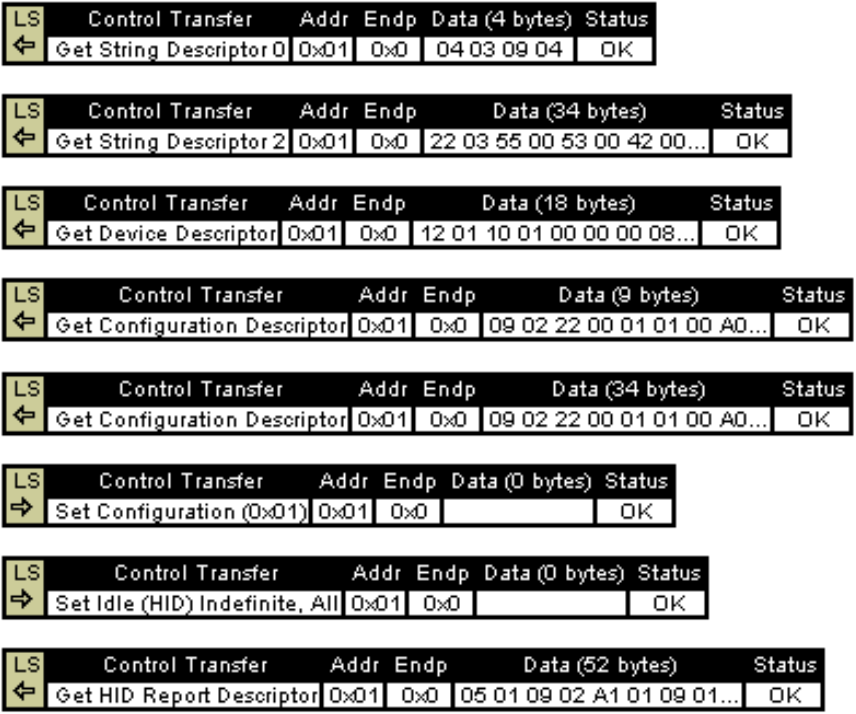
\includegraphics[width=12cm]{img/kap05_graphics_packets}
	\caption{Ukážka grafického vyobrazenia paketov. Obrázok prevzatý zo stránky USB Made Simple~\cite{usbmadesimple_graphics}}
	\label{obr:kap5:graphics_packets}
\end{figure}

\newpage
\section{Pridávanie nových Interpreterov pre descriptory}
Vrámci rozšírenia programu by sme mohli chcieť pridať analýzu pre nové descriptory. V takomto prípade musíme vyriešiť nasledujúce:
\begin{itemize}
\item Definícia descriptoru -- musíme si rozmyslieť odkiaľ zoženieme definíciu daného descriptoru. Môžeme si ho buď nadefinovať sami alebo použiť stávajúce definície z rôznych knižníc. Momentálne si sami definujeme len jeden descriptor -- HID Descriptor a všetky ostatné descriptory ktorých analýzu podporujeme sú definované v súbore usbspec.h.
\item Aby sme vedeli v programe tento druh descriptoru rozpoznať, musíme si pridať jeho číselnú reprezentáciu do enumov:
\begin{enumerate}
\item HeaderDataType -- umožní novú položku v InterpreterFactory.
\item DesriptorTypes -- umožní rozpoznanie daného descriptoru z údajov Setup Paketu. Táto hodnota sa bude musieť presne zhodovať s hodnotou descriptoru definovanou USB špecifikáciou.
\end{enumerate}
\item Definovať v metóde \texttt{ItemManager::GetDataType()} prevod z DescriptorTypes enumu na enum HeaderDataType.
\item Naimplementovať nový Interpreter pre daný descriptor.
\item Pridať do InterpreterFactory možnosť vytvorenia Interpreteru pre daný descriptor.
\end{itemize}
\section{Pridanie Intepreteru pre Interrupt Transfer}
\label{sec:kap5:prid_interrupt}
O analýzu zariadení, ktoré svoje dáta posielajú cez Interrupt Transfer sa momentálne stará InterruptTransferInterpreter, ktorý pôsobí skôr ako ďalšia factory než ako samotný interpreter. Pre pridanie nového zariadenia by sme sa museli postarať o nasledujúce:
\begin{itemize}
\item Číselne zareprezentovať dané zariadenie pridaním novej položky do SupportedDevices enumu.
\item Pridanie tohto zariadenia do našej mapy podporovaných zariadení deviceMap.
\item Pridanie novej položky v metóde \newline\texttt{InterruptTransferInterpreter::Interpret()} v časti kde sa určuje o aké zariadenie sa jedná a na základe toho sa volá daný interpreter.
\item Naimplementovanie nového Interpreteru pre dané zariadenie.
\end{itemize}
\section{Pridanie analýzy pre Isochronous a Bulk \newline Transfer}
\label{sec:kap5:prid_an_iso_bulk}
Momentálne v aplikácii rozpoznávame Isochronous a Bulk transfer len na úrovni hexdumpu, kde jednotlivé bunky zafarbujeme im odpovedajúcim farbám. Aplikácia ale ponúka dostatočne obecný návrh, ktorý umožnuje možnosť pridania aj sémantickej analýzy práve pre tieto typy prenosov. Typ transferu máme uložený v hlavičke paketu a takisto si ho predávame ako parameter v prípade vytvárania novej inštancie \texttt{DataVieweru}. Následne pre interpretovanie zvyškových dát paketu vytvárame novú inštanciu \texttt{AdditionalDataModel}, ktorá používa \texttt{InterpreterFactory} na výber správneho Interpreteru. V tejto factory máme definované položky aj pre Bulk a Isochronous transfer, ktoré ale momentálne vracajú \texttt{nullptr}. Stačí nám teda vytvoriť nový Interpreter práve pre tieto transfery a pridať ho do factory. Je celkom pravdepodobné, že by sme pred interpretovaním jednotlivých zariadení iných prenosov museli najprv zozbierať dáta o formáte ich inputu z descriptorov, ktoré posielajú USB hostovi počas konfigurácie. Pripojenie nového zariadenia na zbernicu a vytvorenie jemu odpovedajúcej štruktúry \texttt{BusDevice} riešime v \texttt{ItemManager::ProcessPacket()} pomocou metódy \texttt{CreateDevice()}. Tá momentálne sekvenčne prechádza dáta paketu a v prípade, že sa jedná o HID/Endpoint/Interface descriptor, vytiahne z nich potrebné dáta. V prípade rozšírenia o nový descriptor je nutné len pridať možnosť rozpoznania tohto typu descriptoru a následne jeho konkrétnu analýzu.
\section{Možnosť rozšírenia na iné platformy}
Hlavná podporovaná platforma našej aplikácie je Windows. V priebehu samotného návrhu sme chceli čo najviac obmedziť viazanie sa na jednu špecifickú platformu, pretože už vtedy sme mohli uvažovať nad prípadným neskôrším rozšírením na iné platformy. To malo za následok niektoré naše rozhodnutia, ako napríklad výber multiplatformového Qt frameworku, alebo manuálne spracovávanie pcap súborov pomocou QFile namiesto použitia Npcap API. S Windowsom nás ale bohužiaľ stále spája zopár vecí, ktoré by sme museli v prípade rozšírenia na iné platformy riešiť inak. Z hľadiska zdrojového kódu to je používanie Windows knižníc. Tie využívame v týchto prípadoch:
\begin{itemize}
\item Pri používaní štruktúr základných descriptorov -- tie sú definované v súbore usbspec.h
\item Štruktúry definované USBPcapom využívajú dátové typy ako napríklad \textit{USHORT}, \textit{USBD\_STATUS}, \textit{UINT32}, ktoré sú definované rôznymi Windows knižnicami.
\end{itemize}

Ďalší problém je s celkovou integráciou nášho programu s USBPcapom, čo je sniffer ktorý funguje iba na Windowse. Spracovanie pcap súborov a formátovanie jednotlivých paketov úzko súvisi s formátom v akom ich USBPcap ukladá.